\documentclass[a4paper,11pt,oneside]{report}

\usepackage[main=french]{babel}
\usepackage[T1]{fontenc}
\usepackage[utf8]{inputenc}
\usepackage{geometry}
\geometry{a4paper, margin=2.3cm, headheight=16pt}
\usepackage{graphicx}
\usepackage{caption}
\usepackage{float}
\usepackage{xcolor}
\usepackage{enumitem}
\usepackage{fancyhdr}
\usepackage{setspace}
\usepackage{hyperref}

\hypersetup{colorlinks=false, pdfborder={0 0 0}}
\setstretch{1.12}
\setlength{\parindent}{1.5em}
\setlength{\parskip}{0.35em}
\setlist[itemize]{label=\textendash, leftmargin=*, nosep}
\captionsetup[figure]{font=footnotesize, justification=justified, singlelinecheck=false}

\newcommand{\reporttype}{Rapport de visualisation scientifique}
\newcommand{\reporttitletext}{Etude de la decompression d'un reservoir avec ParaView}
\newcommand{\reportshorttitle}{Decompression d'un reservoir}
\newcommand{\reportauthor}{Jianye Shi}
\newcommand{\reportprogram}{Master 1 CHPS -- UVSQ}
\newcommand{\reportyear}{Annee universitaire 2025--2026}
\newcommand{\reportdate}{17 avril 2026}

\fancyhf{}
\fancyhead[L]{\textit{\reportshorttitle}}
\fancyhead[R]{Visualisation scientifique}
\fancyfoot[C]{\thepage}
\renewcommand{\headrulewidth}{0.4pt}
\setlength{\headheight}{16pt}

\begin{document}

\pagenumbering{gobble}
\begin{titlepage}
  \centering
  \vspace*{0.8cm}
  
\includegraphics[width=0.75\textwidth]{../Images/ISTY-logo-2025-RVB.jpg}\par
  \vspace{0.9cm}
  {\Large \reportprogram\par}
  \vspace{0.4cm}
  {\large \reportyear\par}
  \vspace{2.2cm}
  {\large \reporttype\par}
  \vspace{0.6cm}
  {\huge\bfseries \reporttitletext\par}
  \vspace{1.2cm}
  {\large Cas \texttt{decompressionTank}\par}
  \vspace{2.2cm}
  \begin{flushleft}
    \textbf{Auteur :} \reportauthor
  \end{flushleft}
  \vfill
  {\large \reportdate\par}
\end{titlepage}

\clearpage
\pagestyle{fancy}
\pagenumbering{arabic}
\setcounter{page}{1}

\section*{Cas et objectif}
Le cas \texttt{decompressionTank} represente un reservoir initialement a haute pression relie a une petite buse laterale. L'objectif du travail est d'observer comment la pression interne diminue au cours du temps et comment cette diminution s'accompagne d'une acceleration du fluide au voisinage de la sortie. Le rapport vise a montrer, a partir de visualisations et de courbes, quels comportements physiques peuvent etre extraits de ce jeu de donnees.

Le champ scalaire principal est la pression \texttt{p} et le champ vectoriel est la vitesse \texttt{U}. L'analyse est construite autour de trois types d'information complementaires : une vue spatiale globale de l'ecoulement, une mise en evidence locale de la zone de sortie et des statistiques superposees qui permettent de comparer plusieurs positions ou plusieurs instants. Cette combinaison est adaptee au bareme, car elle mobilise des filtres et relie directement les images a une interpretation physique.

\begin{figure}[H]
  \centering
  \begin{minipage}[t]{0.32\textwidth}
    \centering
    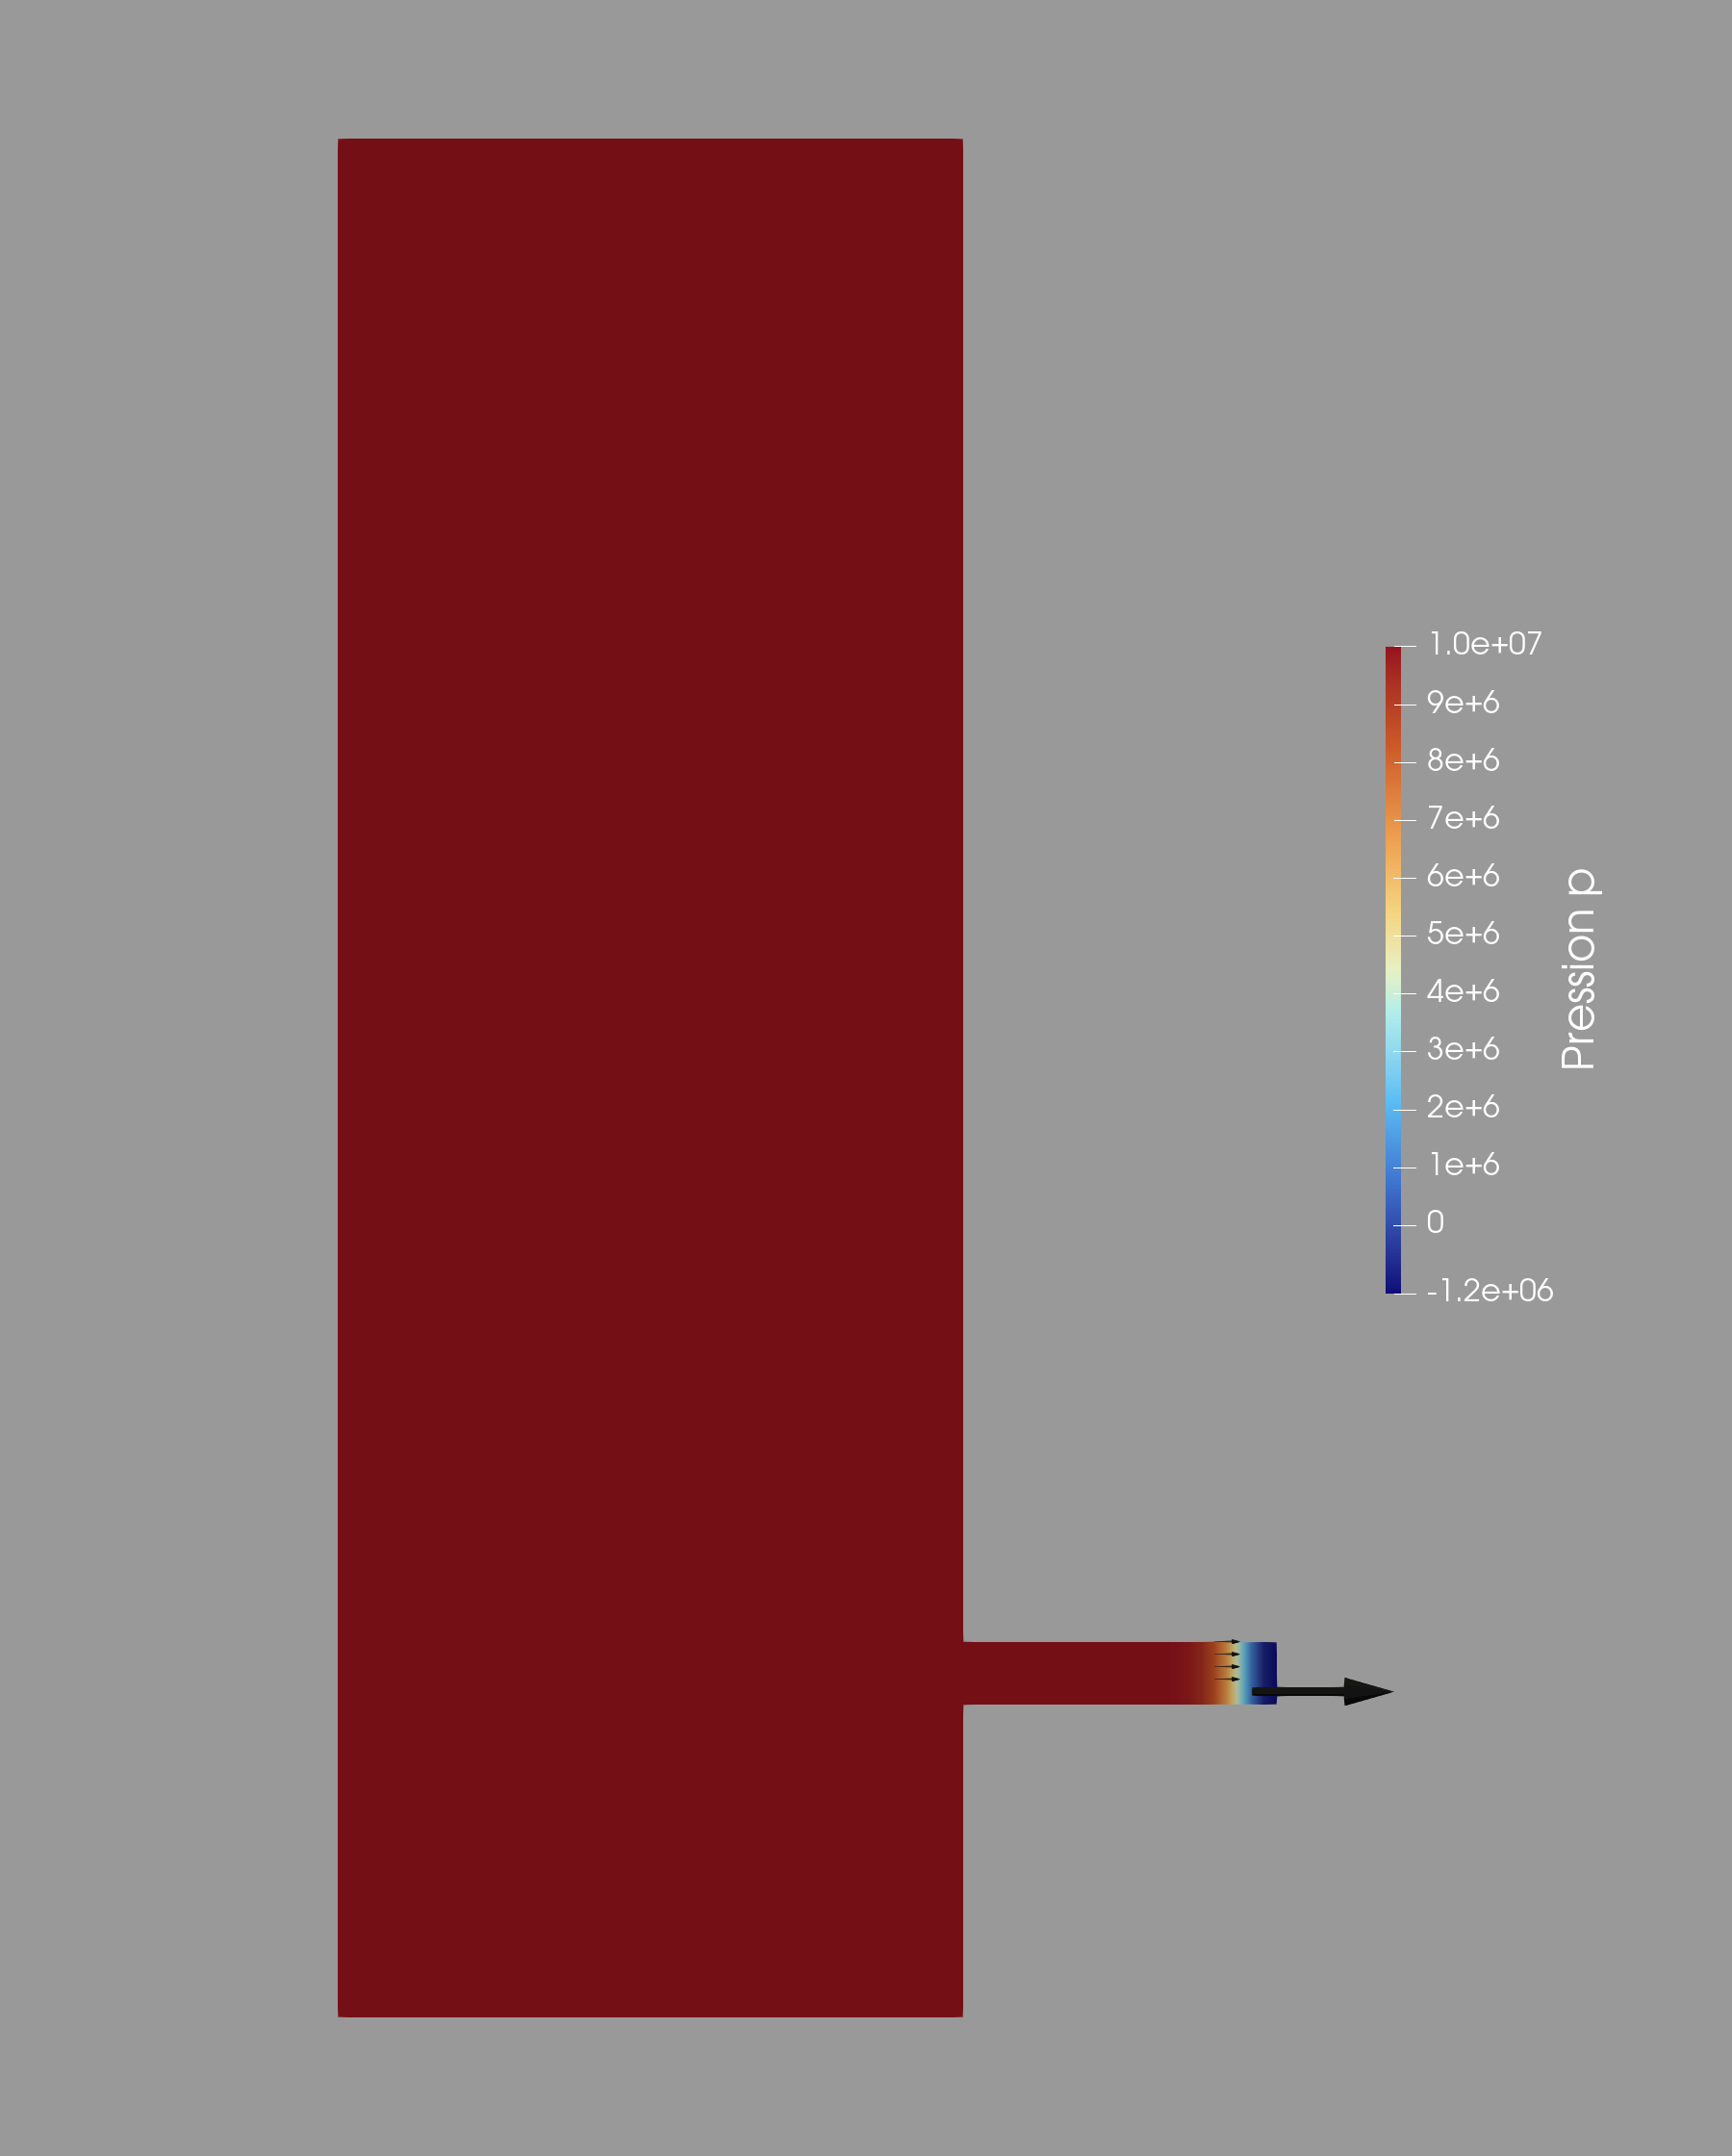
\includegraphics[width=\textwidth]{report_assets/figures/figure1_early.png}
    \caption*{$t = 5.0\times 10^{-6}\ \mathrm{s}$}
  \end{minipage}\hfill
  \begin{minipage}[t]{0.32\textwidth}
    \centering
    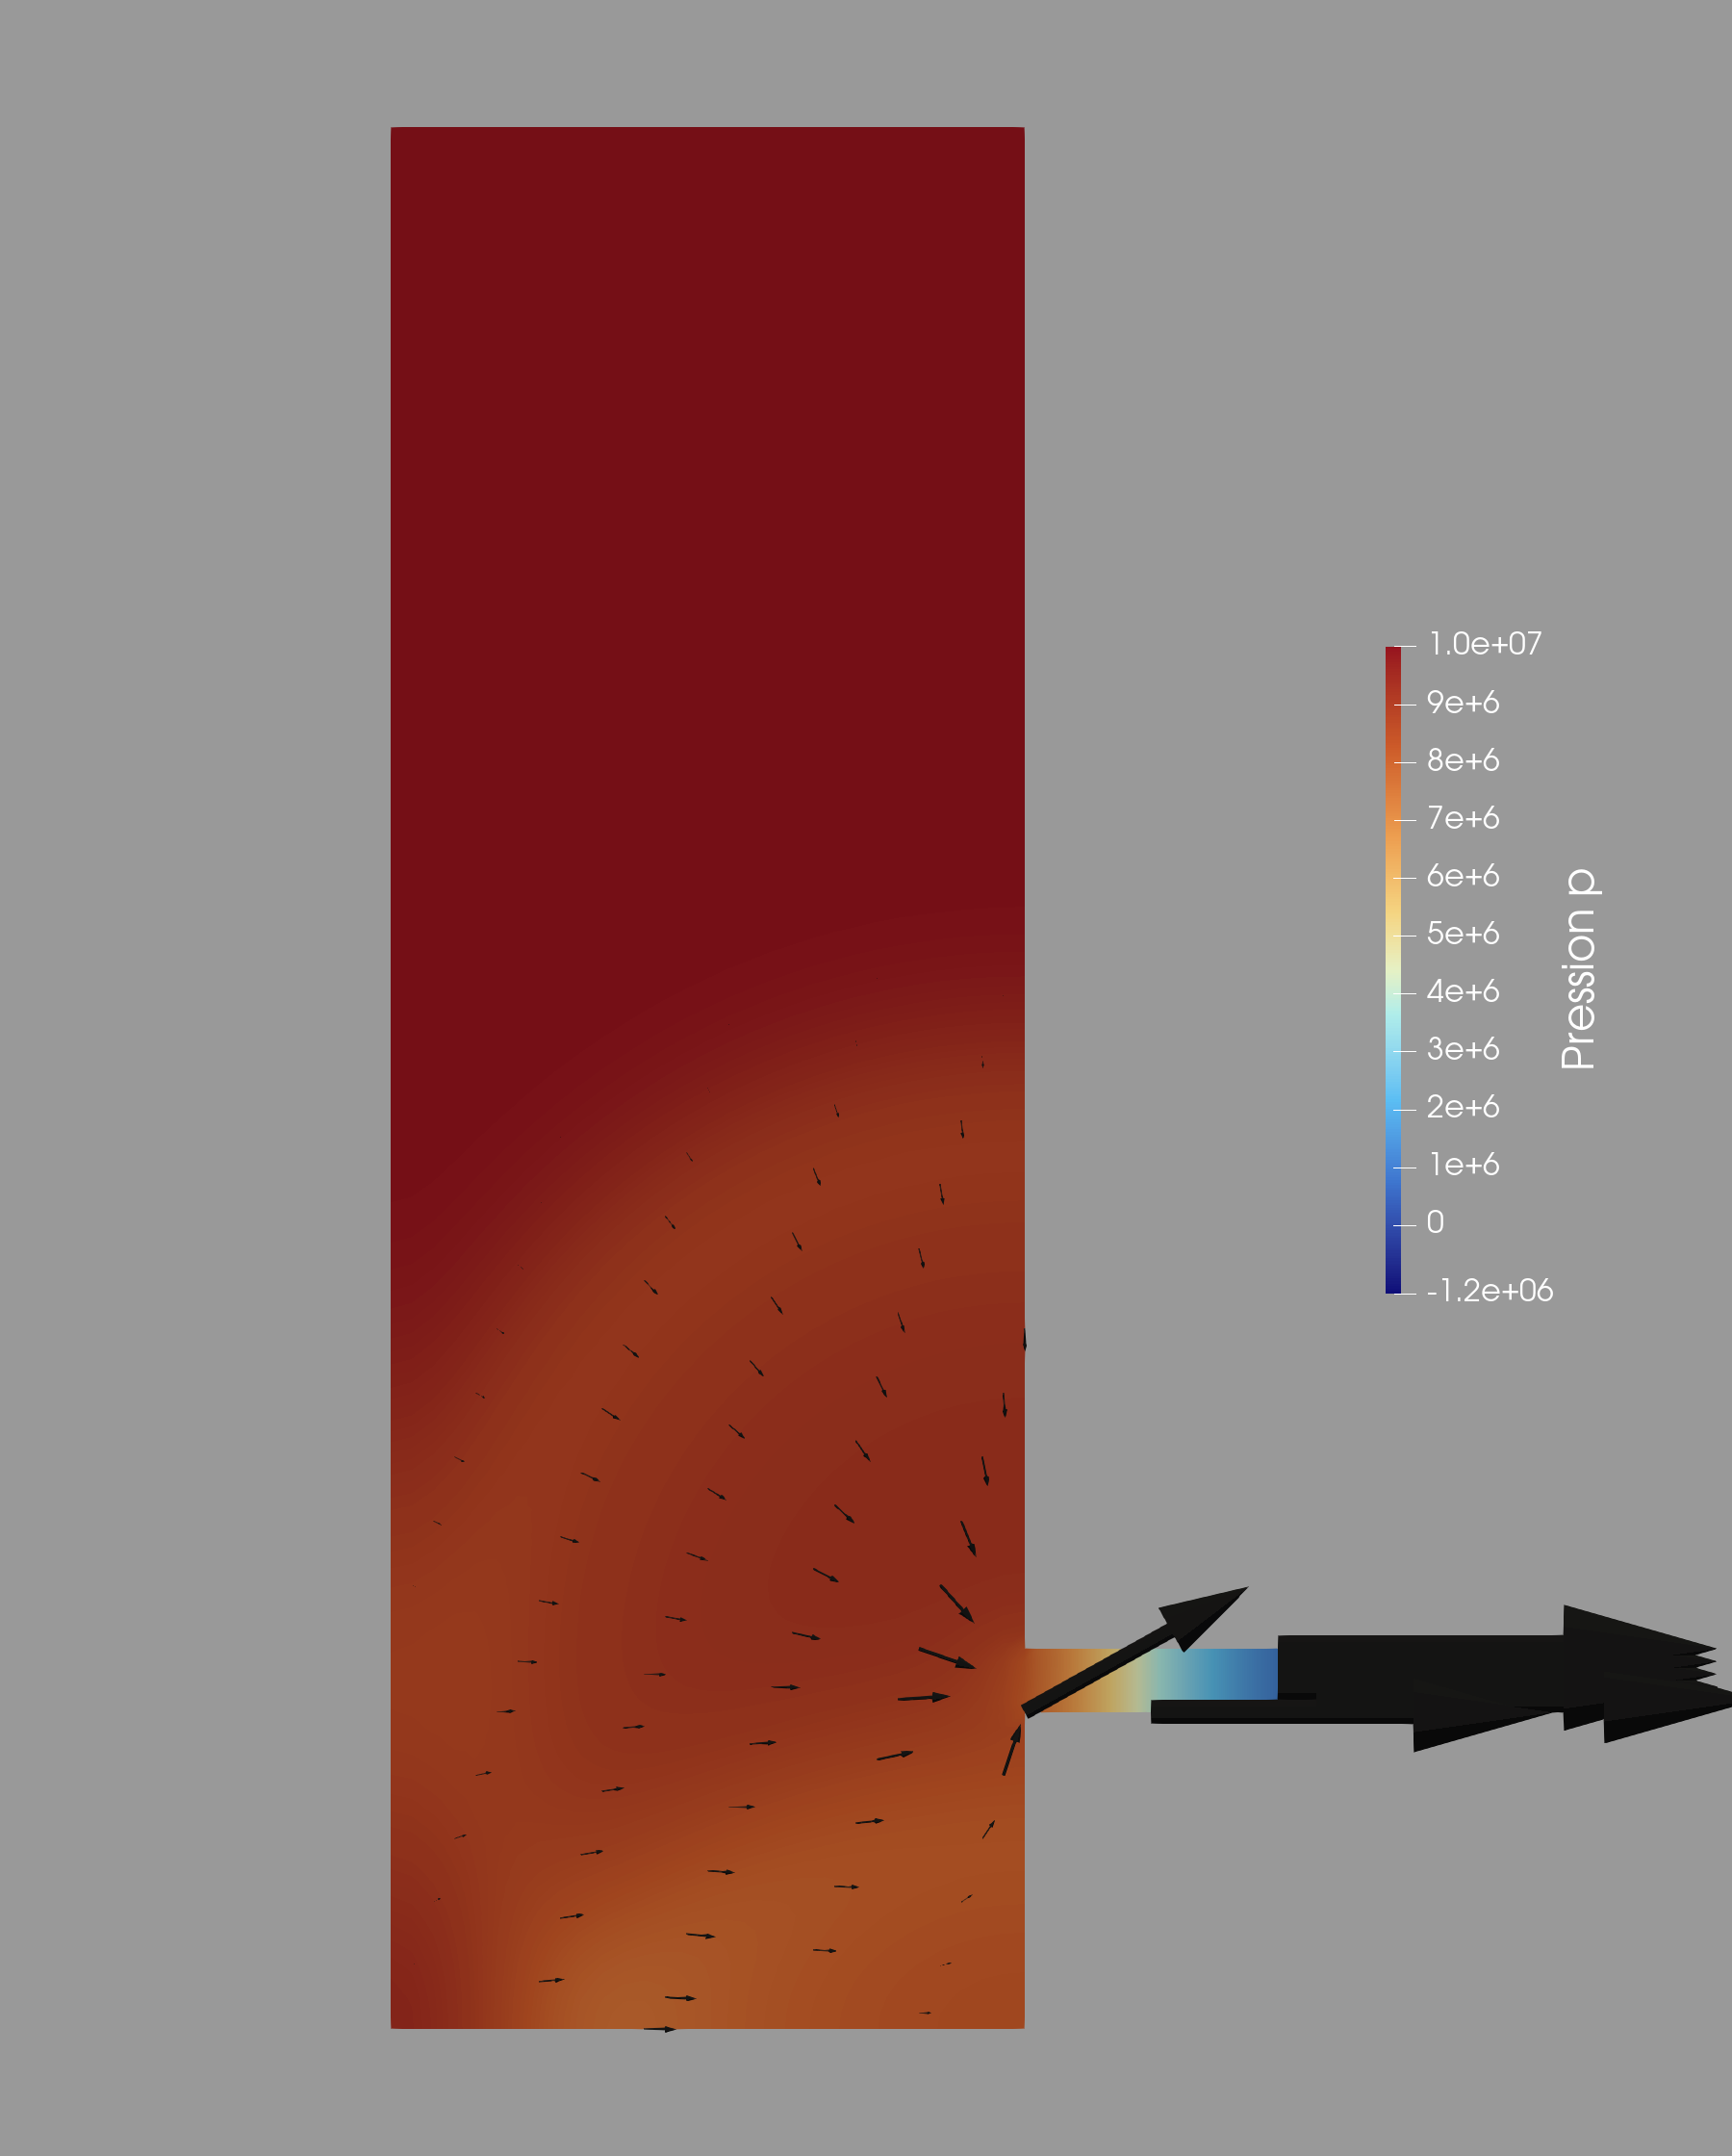
\includegraphics[width=\textwidth]{report_assets/figures/figure1_mid.png}
    \caption*{$t = 1.0\times 10^{-4}\ \mathrm{s}$}
  \end{minipage}\hfill
  \begin{minipage}[t]{0.32\textwidth}
    \centering
    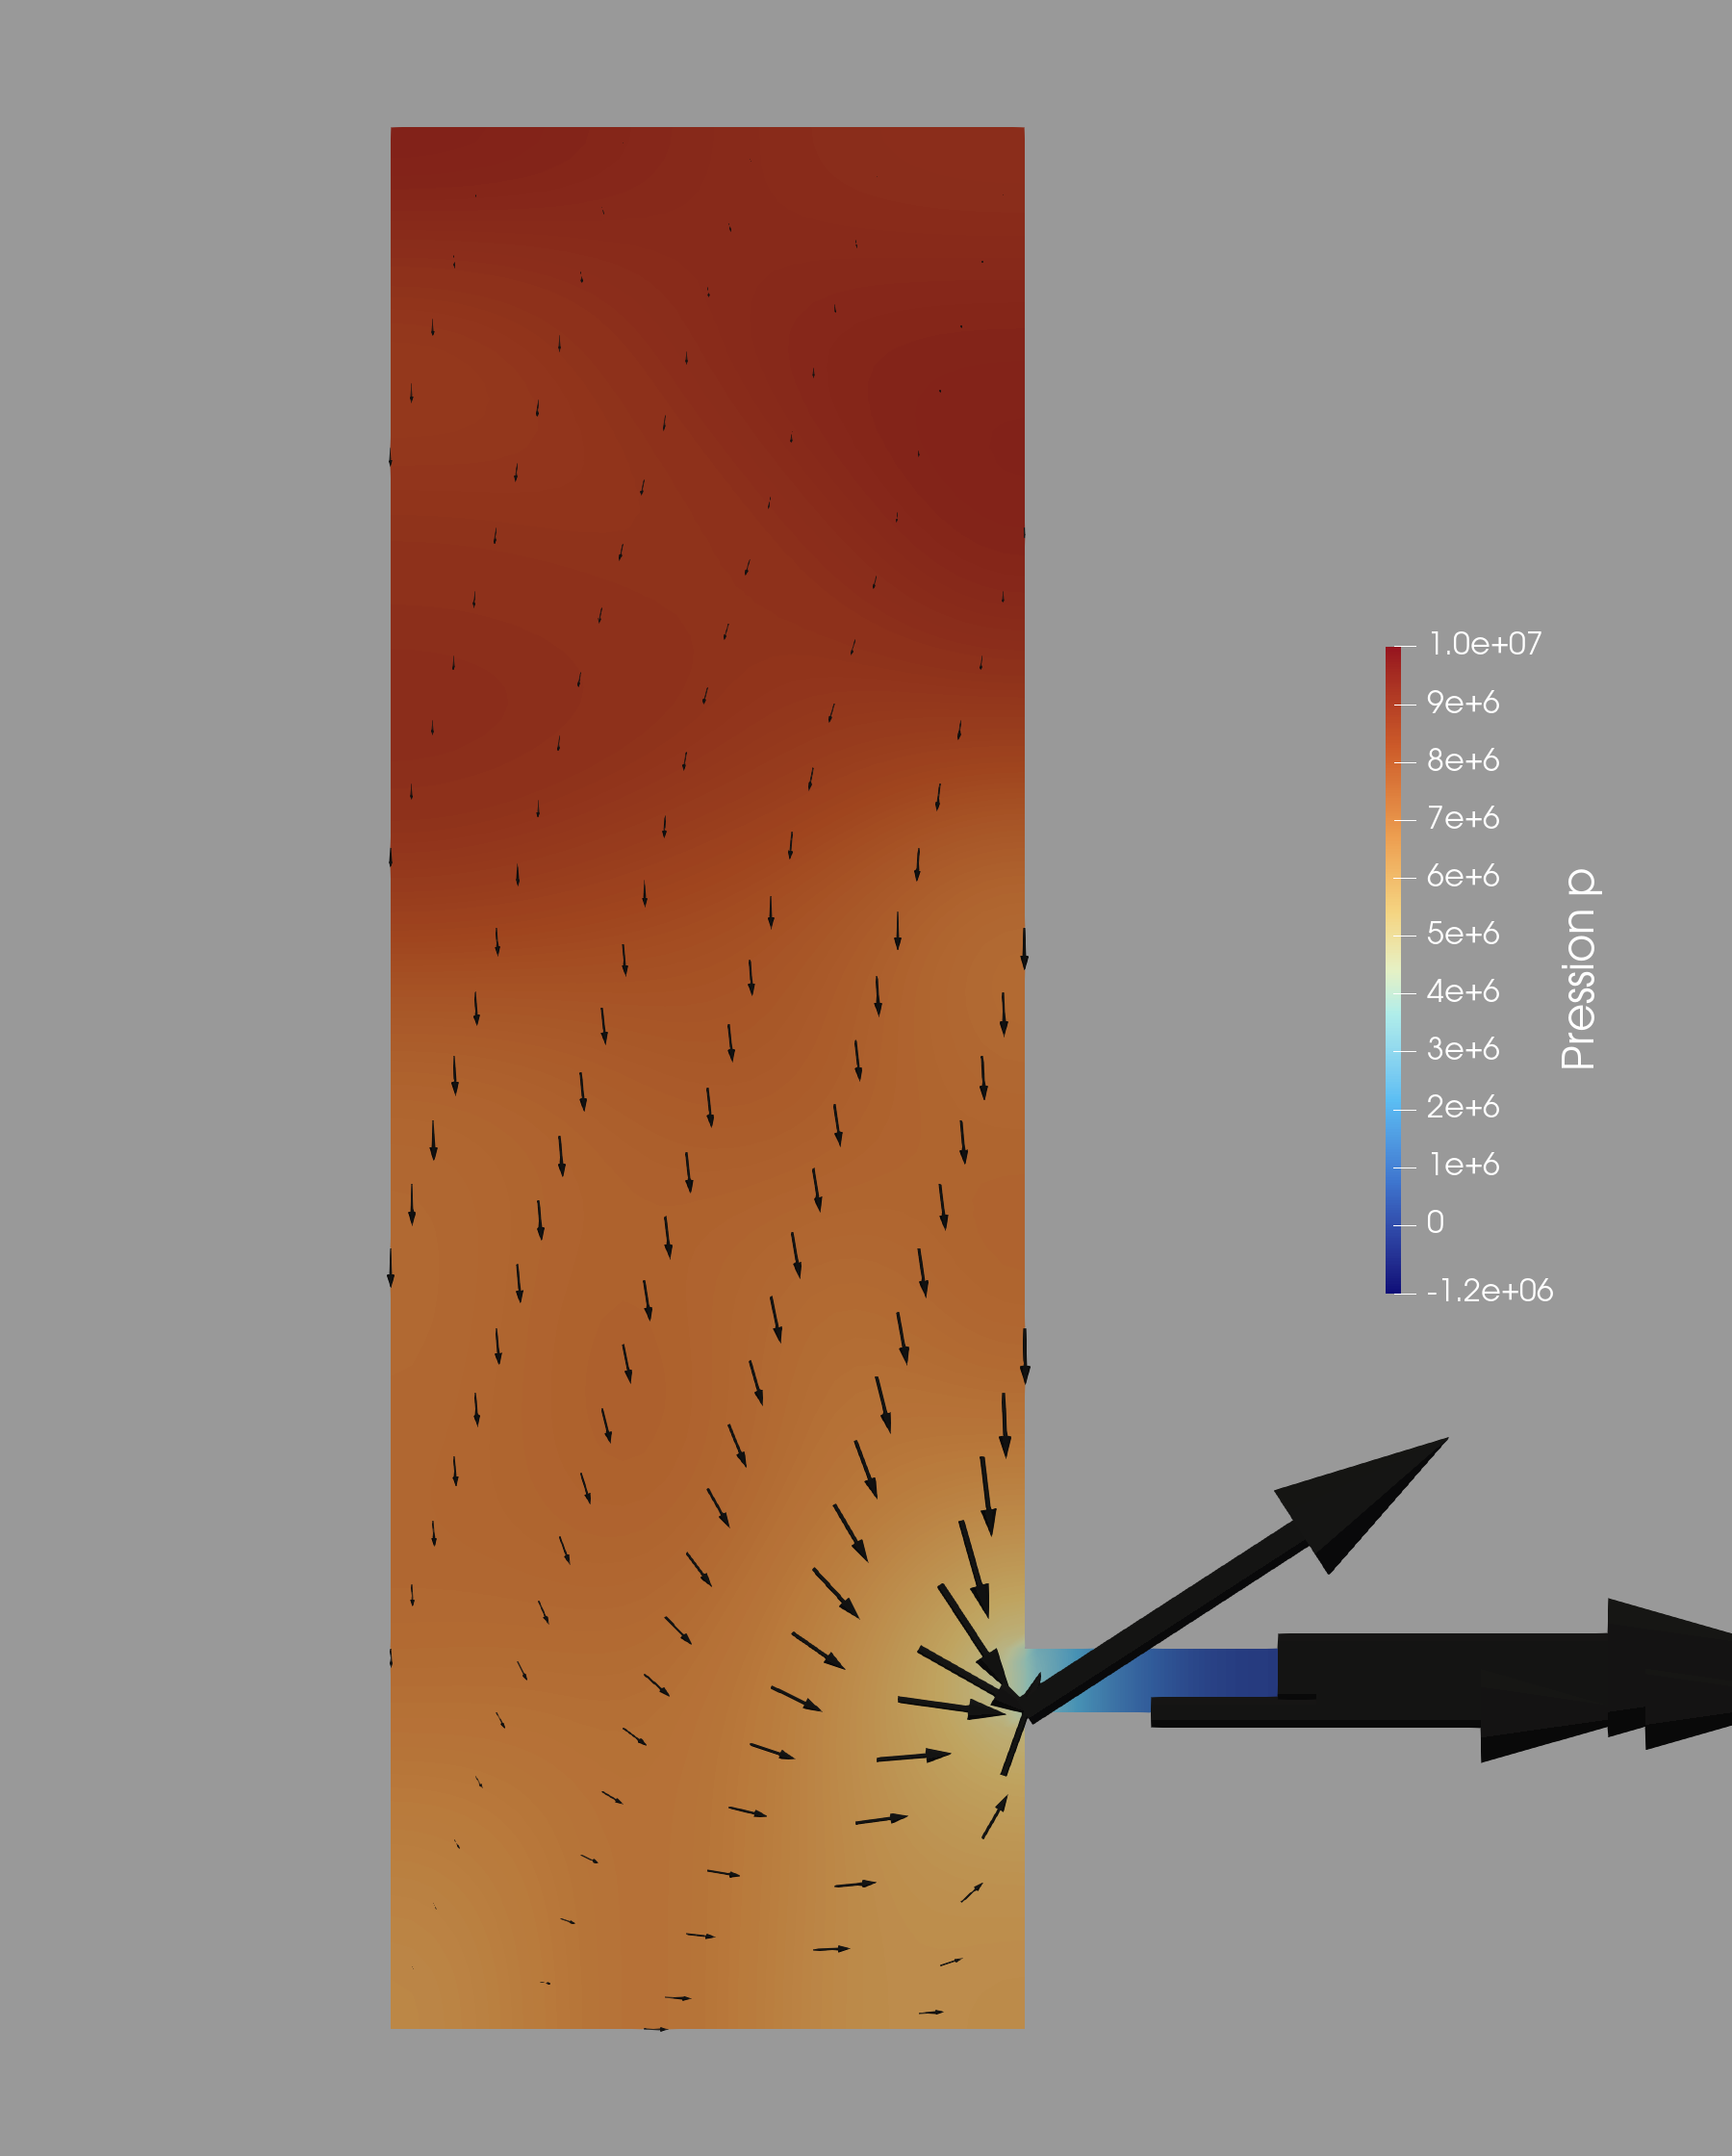
\includegraphics[width=\textwidth]{report_assets/figures/figure1_late.png}
    \caption*{$t = 2.0\times 10^{-4}\ \mathrm{s}$}
  \end{minipage}
  \caption{Vue d'ensemble de la pression et des glyphes de vitesse a trois instants caracteristiques.}
\end{figure}

La figure 1 etablit le cadre general de l'evolution transitoire. Au premier instant, la pression reste presque uniforme dans le reservoir et le champ de vitesse demeure faible. Aux instants suivants, la zone voisine de la buse devient plus contrastee et l'orientation des glyphes vers l'exterieur indique que la reponse de l'ecoulement se structure d'abord autour de la sortie.

\section*{Methodes et filtres utilises}
Toutes les visualisations ont ete produites a partir des sorties VTK du cas
\texttt{decompressionTank}.
Le filtre \texttt{Slice} est utilise sur le plan median \(z=0\), ce qui
fournit une lecture bidimensionnelle d'une geometrie tres mince selon cette
direction. Sur cette coupe centrale, le filtre \texttt{Glyph} est employe pour
representer la direction du vecteur \texttt{U} et une intensite relative de
l'ecoulement, tandis que \texttt{Contour} organise le champ de pression en
lignes isovaleurs afin de rendre plus lisible sa variation spatiale.

Les composantes ParaView utilisees pour l'analyse quantitative sont \texttt{Plot Over Line} et \texttt{Plot Selection Over Time}. La premiere extrait le champ \texttt{p} le long d'une ligne horizontale orientee du reservoir vers la buse, placee dans le meme plan median que la coupe pour permettre une comparaison spatiale directe entre plusieurs instants. La seconde suit l'evolution de \texttt{p} en deux positions representatives, l'une dans le reservoir et l'autre pres de la sortie, afin de comparer deux reponses locales de nature differente. Enfin, la video combine une vue spatiale a gauche et une courbe temporelle a droite, avec une annotation de temps constante.

\begin{figure}[H]
  \centering
  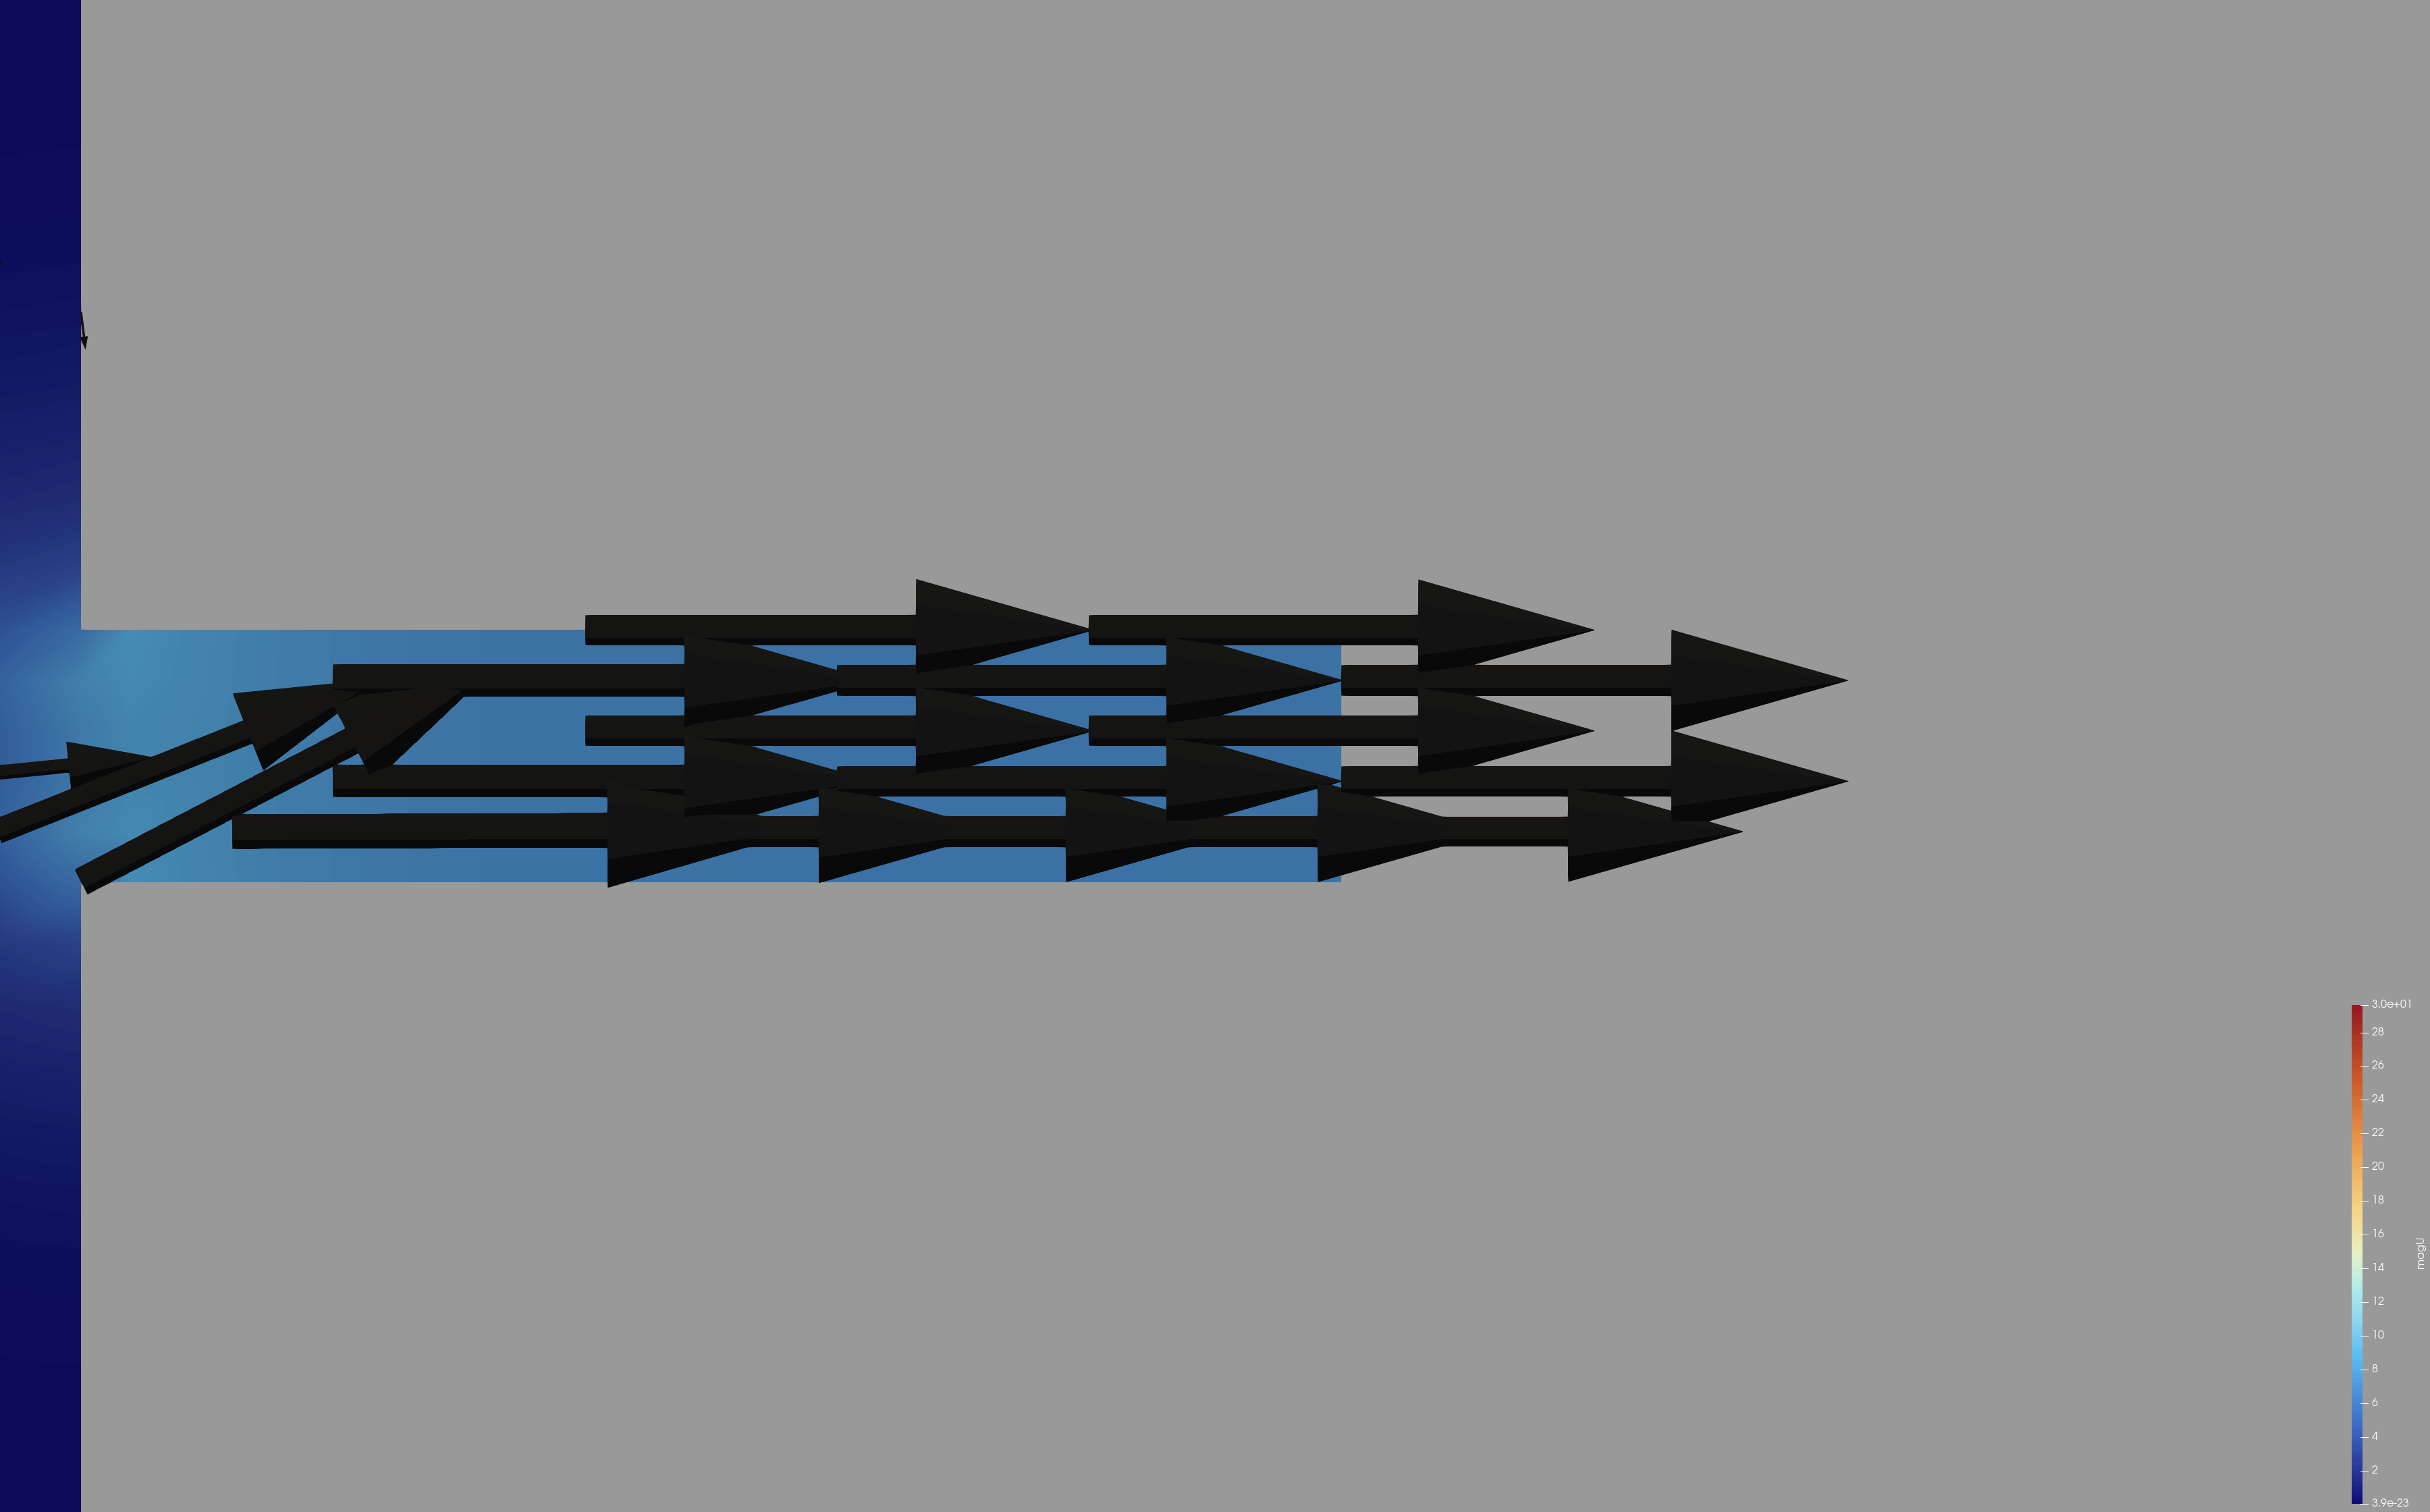
\includegraphics[width=0.77\textwidth]{report_assets/figures/figure2_nozzle_magu.png}
  \caption{Zone de la buse coloree par la norme de la vitesse \texttt{|U|}.}
\end{figure}

Cette vue repond a une question locale : ou l'ecoulement se renforce-t-il et dans quelle direction s'organise-t-il? La figure 2 correspond a un instant precoce du transitoire, choisi pour rendre plus lisible la mise en place de l'acceleration pres de la sortie. La vitesse elevee reste concentree dans une region reduite autour de la buse, alors que le reste du domaine n'atteint pas la meme intensite. Les glyphes orientent cette lecture en indiquant un mouvement principalement dirige vers l'exterieur ; combines au champ de pression observe par ailleurs, ils soutiennent l'interpretation d'une acceleration localisee au voisinage de la buse.

\section*{Resultats et interpretation}
\begin{figure}[H]
  \centering
  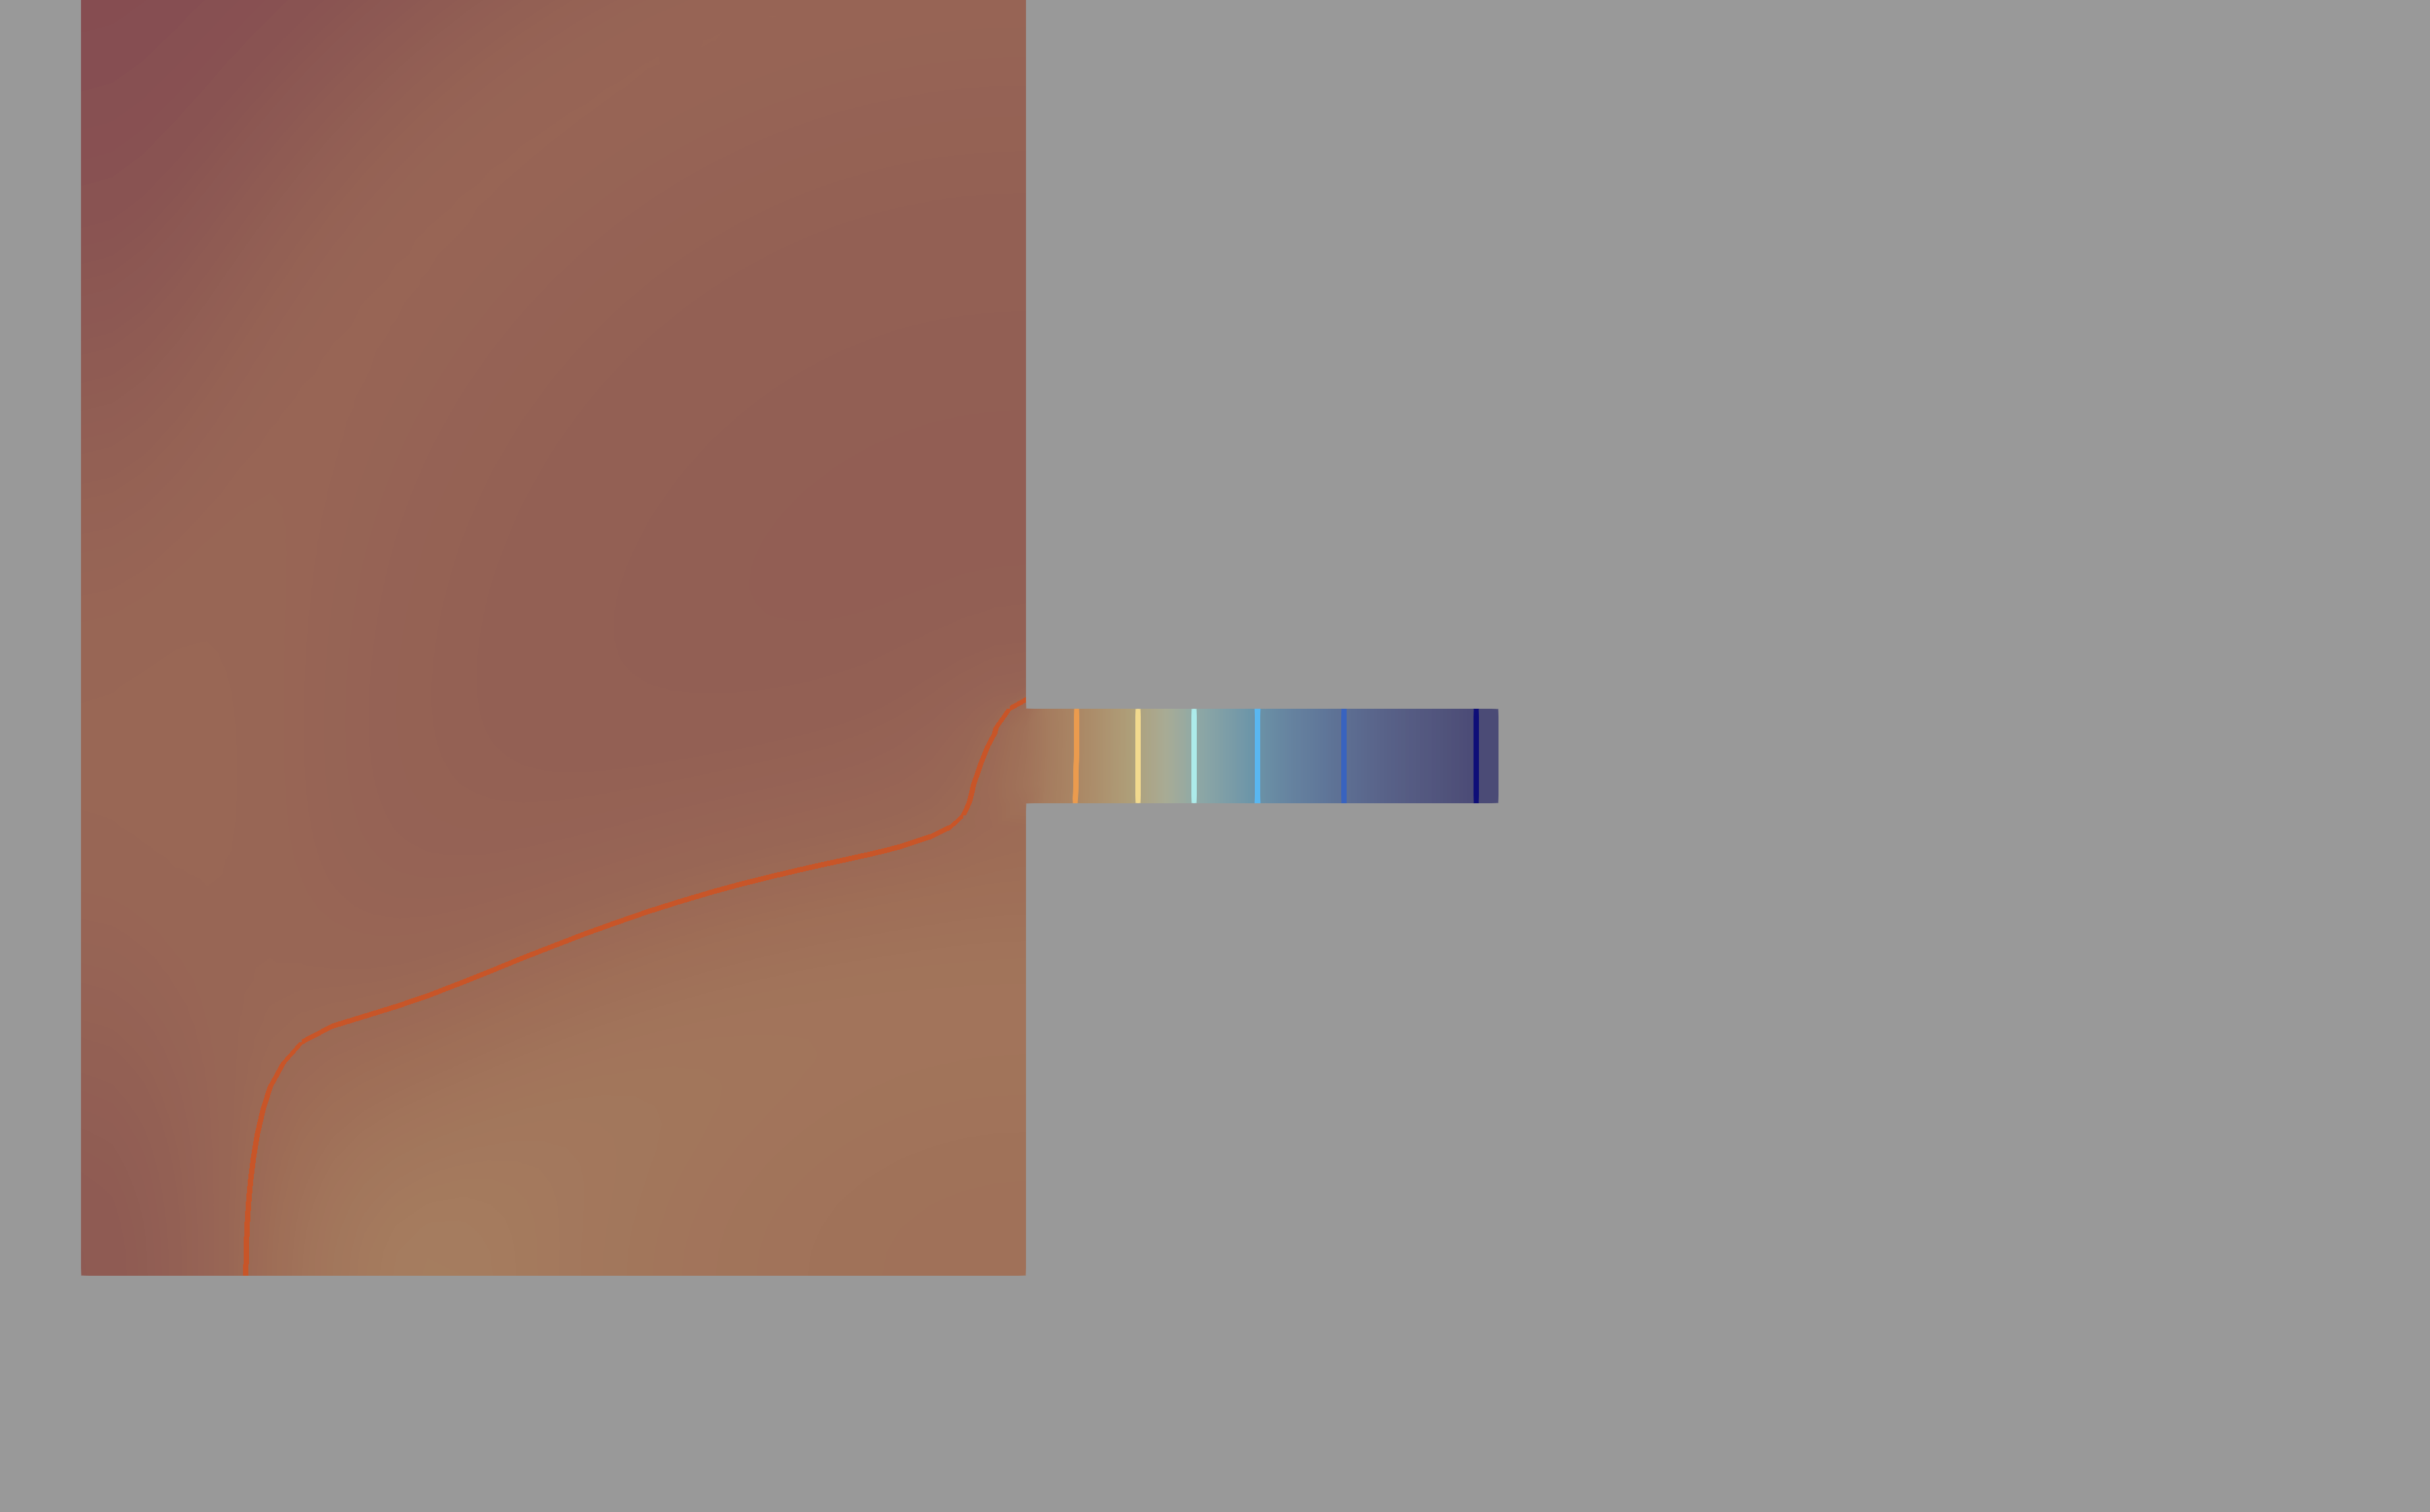
\includegraphics[width=0.82\textwidth]{report_assets/figures/figure3_contours.png}
  \caption{Isovaleurs de pression dans la region de la sortie.}
\end{figure}

La figure 3 repond a une autre question, cette fois sur la structure du champ scalaire : ou la variation de pression est-elle la plus concentree? Au voisinage de la buse, les isovaleurs deviennent nettement plus resserrees que dans le reste du reservoir. Dans une lecture qualitative de ce type, un tel rapprochement des lignes est compatible avec un gradient spatial plus marque ; la figure localise donc la zone ou la transition de pression semble la plus forte, sans se confondre avec l'information cinematique deja portee par la figure 2.

\begin{figure}[H]
  \centering
  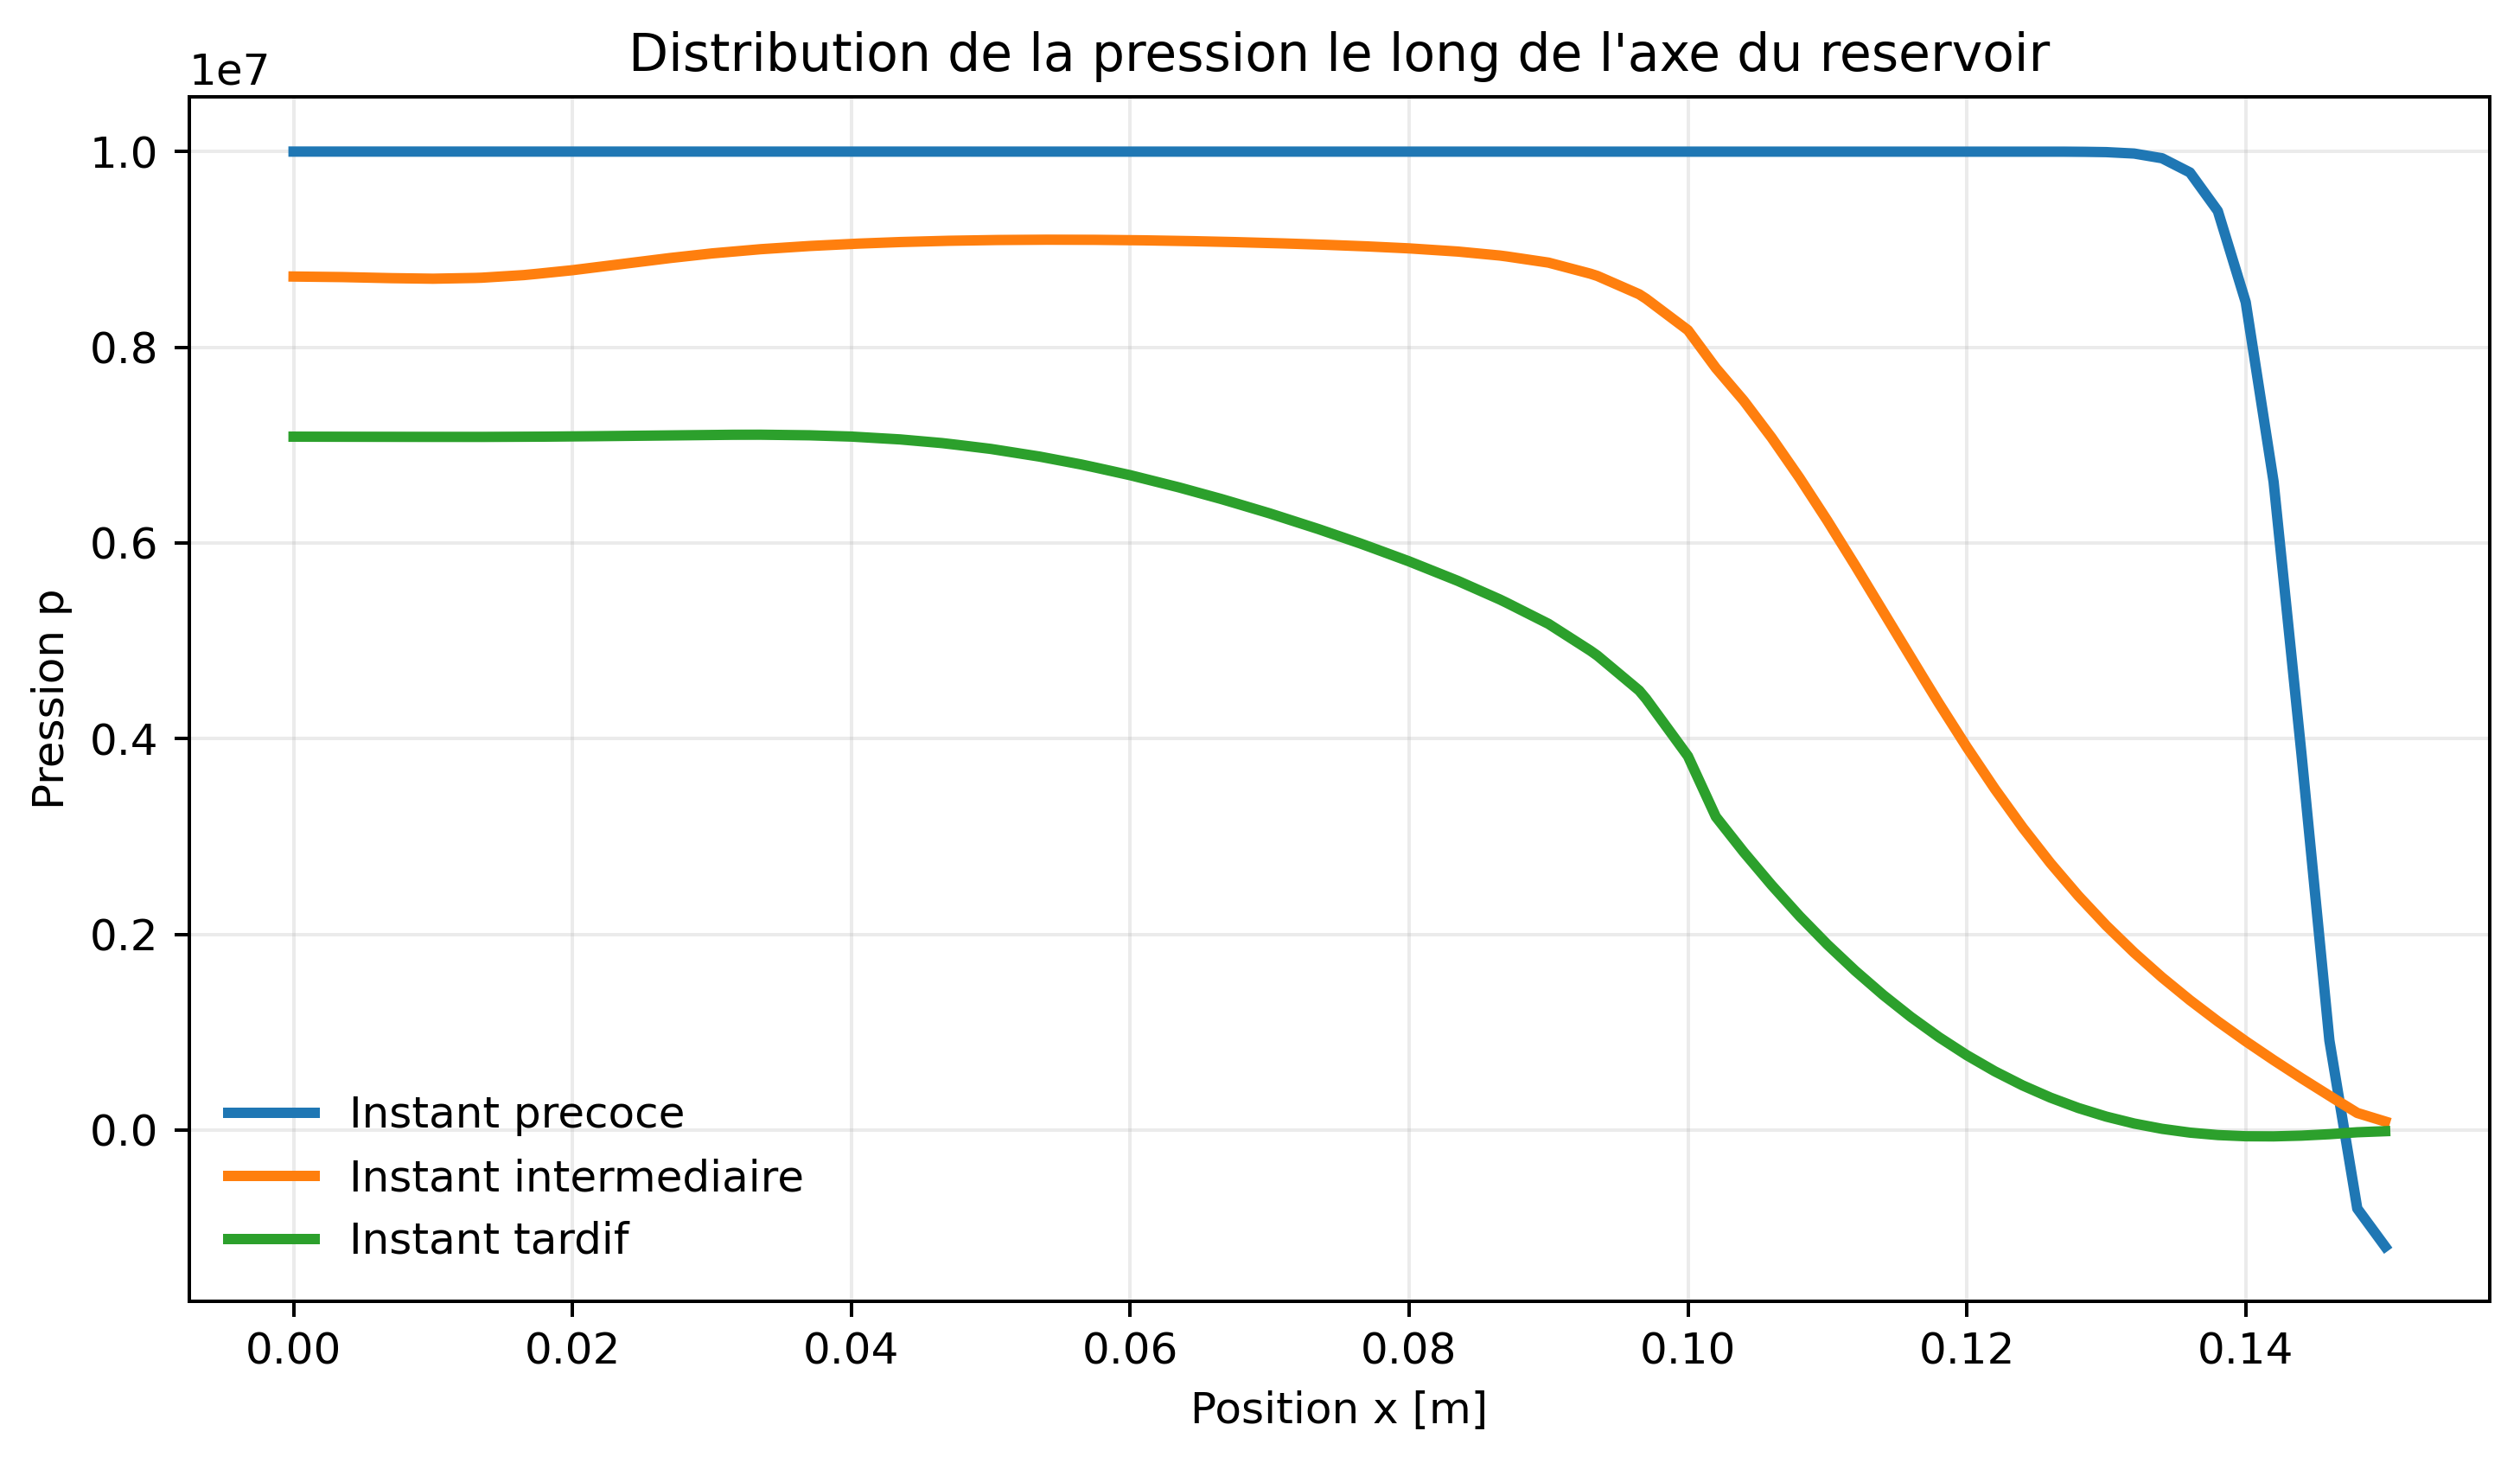
\includegraphics[width=0.76\textwidth]{report_assets/figures/figure4_line_plot.png}
  \caption{Distribution de la pression le long de l'axe horizontal \(y = 0{,}055\ \mathrm{m}\).}
\end{figure}

La figure 4 apporte une comparaison de type profil spatial. Le long de la ligne horizontale reliant l'interieur du reservoir a la zone de sortie, la courbe initiale reste presque plate, tandis que les courbes plus tardives se distinguent surtout dans la partie proche de la sortie. L'ecart entre les instants y devient le plus visible, alors qu'il reste plus limite en amont dans le reservoir ; cette repartition spatiale soutient l'idee d'une decompression non uniforme.

\begin{figure}[H]
  \centering
  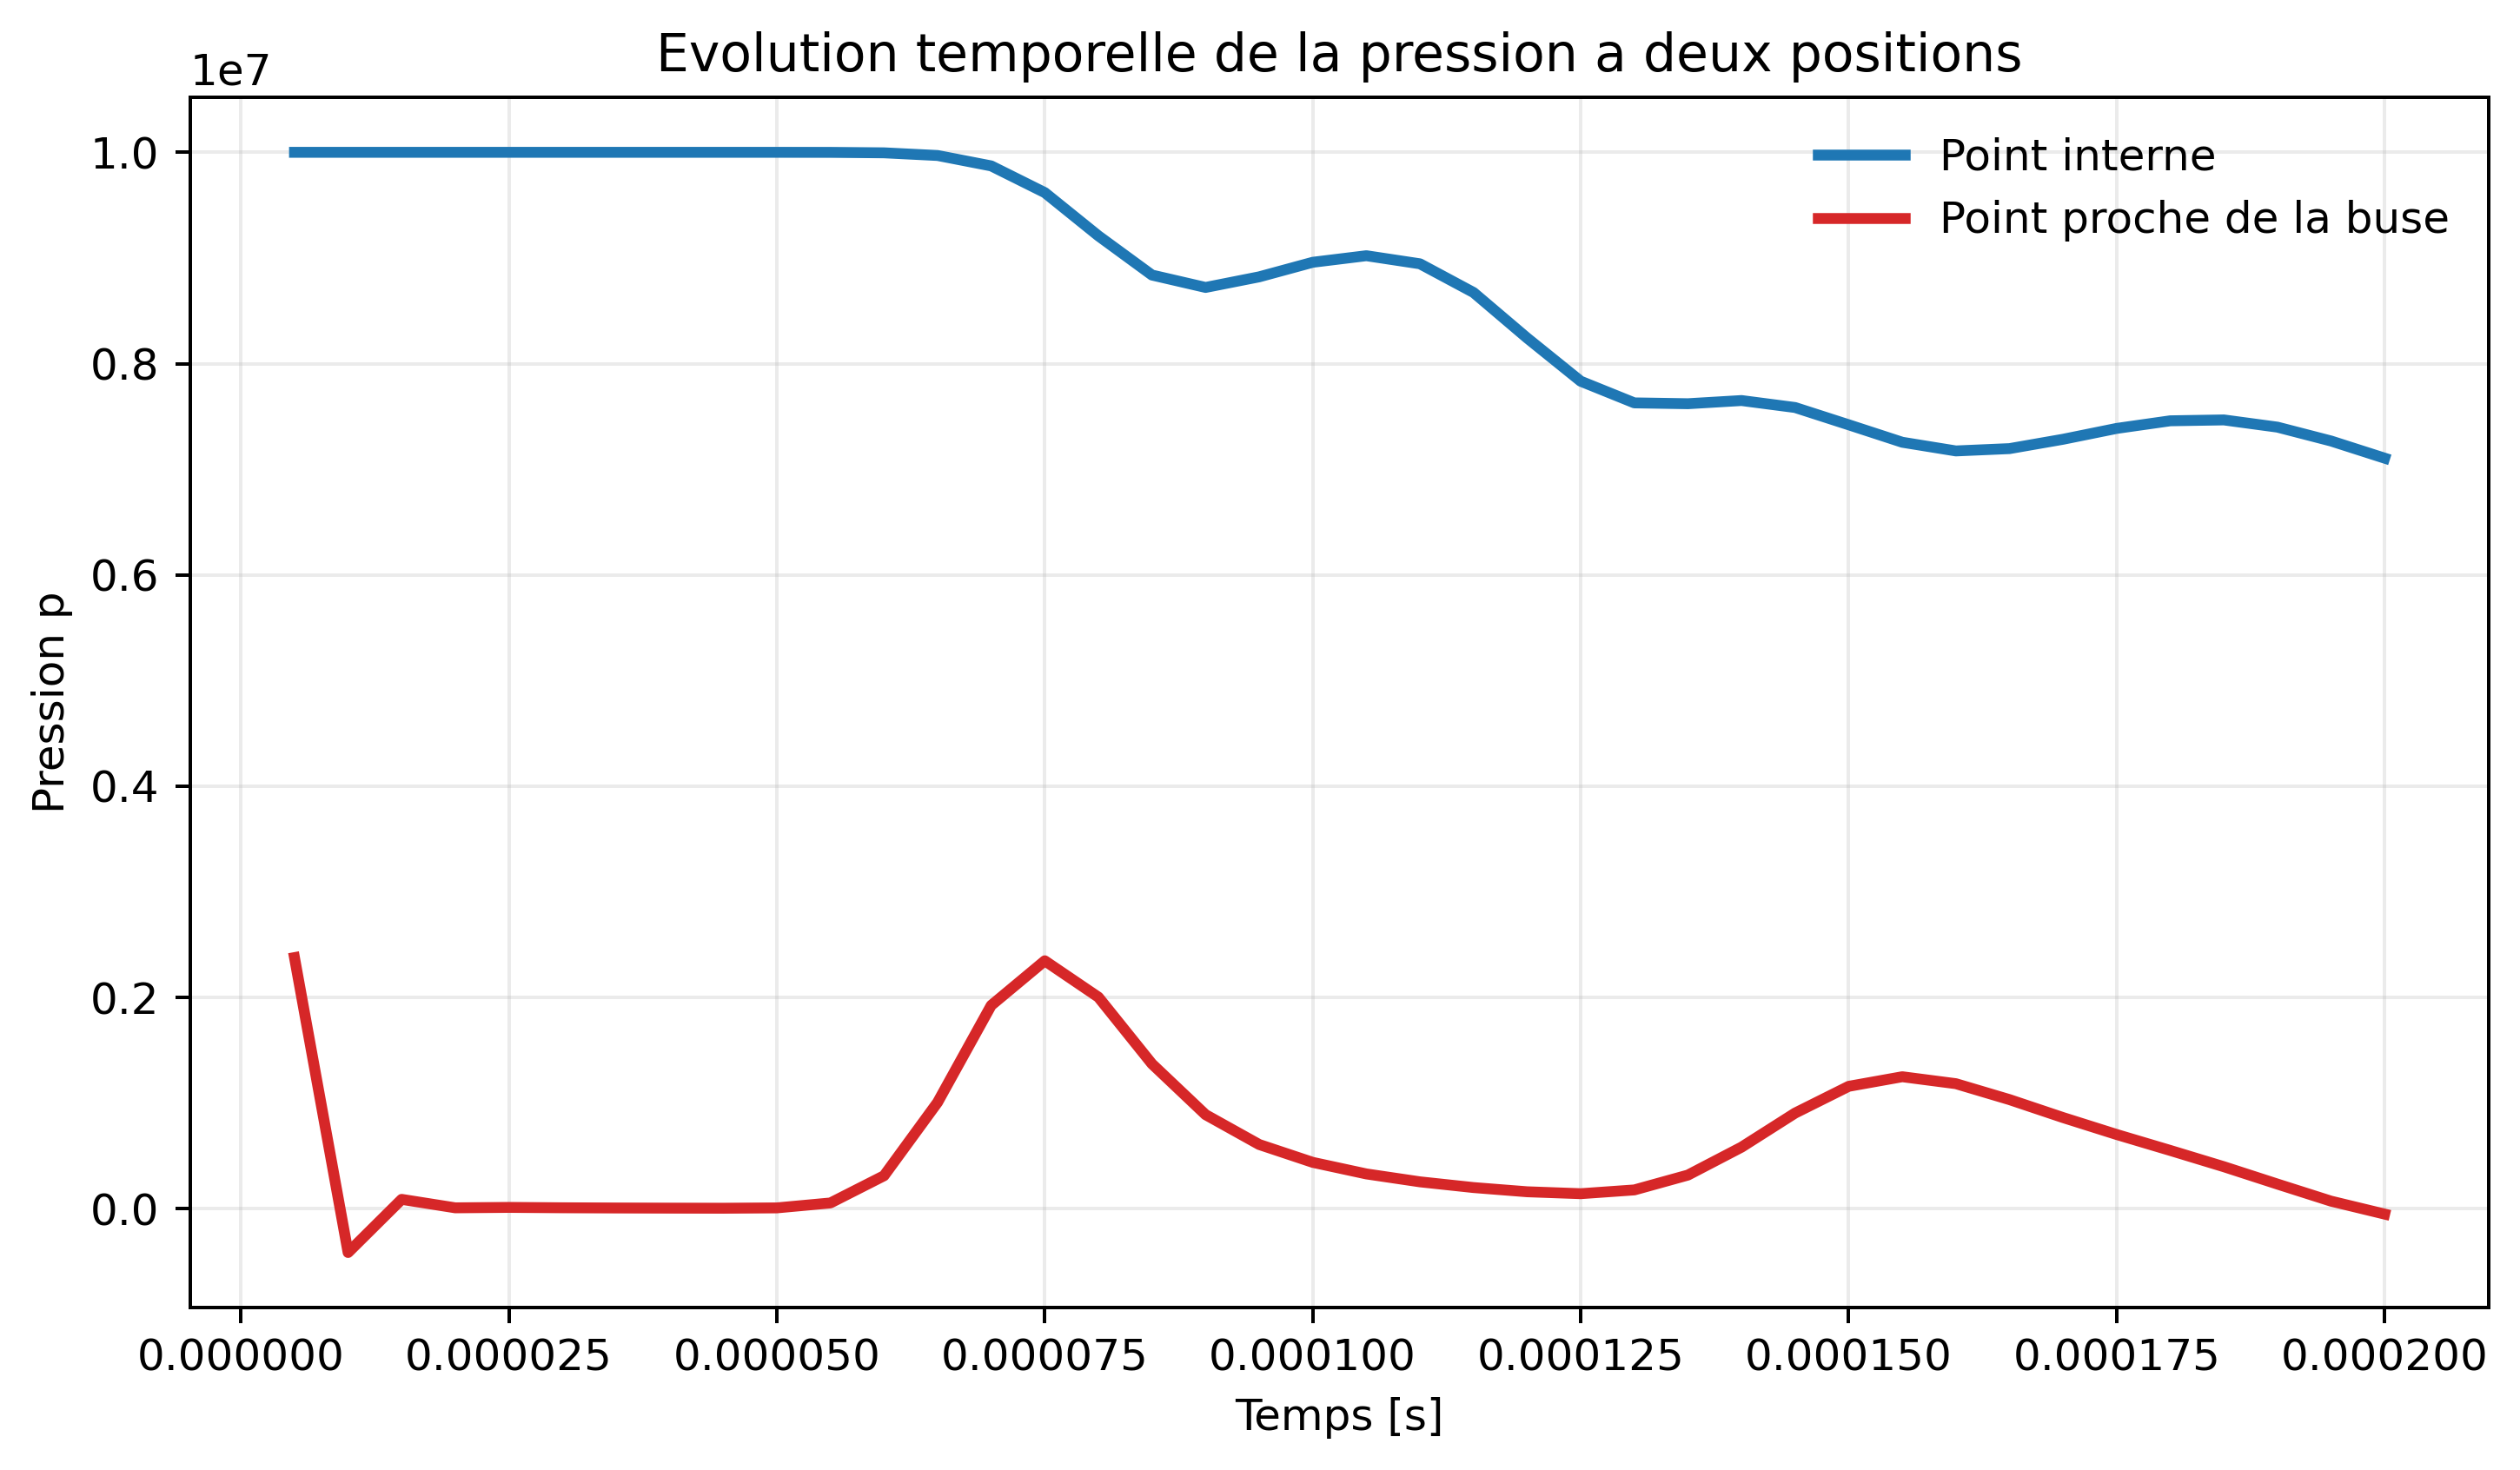
\includegraphics[width=0.76\textwidth]{report_assets/figures/figure5_probe_plot.png}
  \caption{Evolution temporelle de la pression en un point interne et en un point proche de la buse.}
\end{figure}

La figure 5 fournit la lecture temporelle complementaire a la coupe precedente. Le point interne conserve pendant une duree notable une pression elevee avant de diminuer progressivement, tandis que le point proche de la buse presente plus tot une reponse rapide, suivie d'une remontee partielle au cours du transitoire. Cette difference de chronologie entre deux positions representatives indique que les diverses regions du domaine ne repondent pas au meme rythme ; elle va dans le meme sens que les observations spatiales centrees sur la sortie.

La video associee reprend cette lecture sous forme dynamique. La vue de gauche montre l'evolution du champ de pression et des vecteurs de vitesse, tandis que la vue de droite affiche la pression en fonction du temps aux deux positions choisies. La video montre l'evolution transitoire de la decompression dans le reservoir ainsi que la reponse en pression a deux positions representatives.

\section*{Conclusion}
L'etude du cas \texttt{decompressionTank} indique d'abord une diminution globale de la pression dans le reservoir au cours du temps. Elle suggere ensuite que la region de la buse joue un role central dans la dynamique observee : c'est la que les variations spatiales de pression paraissent les plus concentrees et que la reponse du champ de vitesse est la plus visible. Enfin, les courbes superposees montrent que la reponse temporelle pres de la sortie est plus rapide que celle du point interne.

Pris ensemble, les vues spatiales, les isovaleurs et les statistiques temporelles et spatiales soutiennent donc une interpretation coherente : la decompression ne semble pas se distribuer uniformement dans le reservoir, mais s'organise principalement autour de la zone de sortie. Cette lecture repose toutefois sur la coupe mediane, la vue locale de la sortie, un profil spatial et deux positions representatives ; elle decrit donc surtout les tendances dominantes, sans pretendre couvrir l'ensemble des details tridimensionnels.

\end{document}
